% !Mode:: "TeX:UTF-8"
% !TEX program = xelatex

%%%%%%%%%% Port for macOS %%%%%%%%%%%
% Modified: Qin Yubo

\def\usewhat{xelatex}
\documentclass[12pt,openany,oneside]{ctexbook}
                                                     % 本科生毕业论文通常采用单页排版
% !Mode:: "TeX:UTF-8"
%  Authors: 张井   Jing Zhang: prayever@gmail.com     天津大学2010级管理与经济学部信息管理与信息系统专业硕士生
%           余蓝涛 Lantao Yu: lantaoyu1991@gmail.com  天津大学2008级精密仪器与光电子工程学院测控技术与仪器专业本科生

%%%%%%%%%% Package %%%%%%%%%%%%
\usepackage{CJK}
\usepackage{lmodern}
\usepackage[T1]{fontenc}
\usepackage{graphicx}                       % 支持插图处理
\usepackage[a4paper,top= 27.5true mm,left=35.7 true mm,right=27.7 true mm,bottom=25.4true mm,headsep=5.3true mm,foot=5.9true mm]{geometry}
                                            % 支持版面尺寸设置
\usepackage[squaren]{SIunits}               % 支持国际标准单位

\usepackage{titlesec}                       % 控制标题的宏包
\usepackage{titletoc}                       % 控制目录的宏包
\usepackage{fancyhdr}                       % fancyhdr宏包 支持页眉和页脚的相关定义
%\usepackage{ctex}                     % 支持中文显示
\usepackage{CJKpunct}                       % 精细调整中文的标点符号
\usepackage{color}                          % 支持彩色
\usepackage{amsmath}                        % AMSLaTeX宏包 用来排出更加漂亮的公式
\usepackage{amssymb}                        % 数学符号生成命令
\usepackage[below]{placeins}    %允许上一个section的浮动图形出现在下一个section的开始部分,还提供\FloatBarrier命令,使所有未处理的浮动图形立即被处理
\usepackage{multirow}                       % 使用Multirow宏包,使得表格可以合并多个row格
\usepackage{booktabs}                       % 表格,横的粗线;\specialrule{1pt}{0pt}{0pt}
\usepackage{longtable}                      % 支持跨页的表格。
\usepackage{tabularx}                       % 自动设置表格的列宽
\usepackage{subfigure}                      % 支持子图 %centerlast 设置最后一行是否居中
\usepackage[subfigure]{ccaption}            % 支持子图的中文标题
\usepackage[sort&compress,numbers]{natbib}  % 支持引用缩写的宏包
\usepackage{enumitem}                       % 使用enumitem宏包,改变列表项的格式
\usepackage{calc}                           % 长度可以用+ - * / 进行计算
\usepackage{txfonts}                        % 字体宏包
\usepackage{bm}                             % 处理数学公式中的黑斜体的宏包
\usepackage[amsmath,thmmarks,hyperref]{ntheorem}  % 定理类环境宏包,其中 amsmath 选项用来兼容 AMS LaTeX 的宏包
\usepackage{CJKnumb}                        % 提供将阿拉伯数字转换成中文数字的命令
\usepackage{indentfirst}                    % 首行缩进宏包
\usepackage{CJKutf8}                        % 用在UTF8编码环境下,它可以自动调用CJK,同时针对UTF8编码作了设置
%\usepackage{hypbmsec}                      % 用来控制书签中标题显示内容
\newcommand{\tabincell}[2]{\begin{tabular}{@{}#1@{}}#2\end{tabular}}
\usepackage{xcolor}
%支持代码环境
\usepackage{listings}
\lstset{numbers=left,
language=[ANSI]{C},
numberstyle=\tiny,
extendedchars=false,
showstringspaces=false,
breakatwhitespace=false,
breaklines=true,
captionpos=b,
keywordstyle=\color{blue!70},
commentstyle=\color{red!50!green!50!blue!50},
frame=shadowbox,
rulesepcolor=\color{red!20!green!20!blue!20}
}
%支持算法环境
\usepackage[boxed,ruled,lined]{algorithm2e}
\usepackage{algorithmic}

\usepackage{array}
\newcommand{\PreserveBackslash}[1]{\let\temp=\\#1\let\\=\temp}
\newcolumntype{C}[1]{>{\PreserveBackslash\centering}p{#1}}
\newcolumntype{R}[1]{>{\PreserveBackslash\raggedleft}p{#1}}
\newcolumntype{L}[1]{>{\PreserveBackslash\raggedright}p{#1}}

\def\atemp{xelatex}\ifx\atemp\usewhat
\usepackage[unicode,
            pdfstartview=FitH,
            bookmarksnumbered=true,
            bookmarksopen=true,
            colorlinks=false,
            pdfborder={0 0 1},
            citecolor=blue,
            linkcolor=red,
            anchorcolor=green,
            urlcolor=blue,
            breaklinks=true
            ]{hyperref}
\fi
                                % 定义本文所使用宏包
\graphicspath{{figures/}}                            % 定义所有的图像文件在 figures 子目录下
\begin{document}                                     % 开始全文
% !Mode:: "TeX:UTF-8"
%  Authors: 张井   Jing Zhang: prayever@gmail.com     天津大学2010级管理与经济学部信息管理与信息系统专业硕士生
%           余蓝涛 Lantao Yu: lantaoyu1991@gmail.com  天津大学2008级精密仪器与光电子工程学院测控技术与仪器专业本科生

%%%%%%%%%%%%%%%%% Fonts Definition and Basics %%%%%%%%%%%%%%%%%
%\newcommand{\song}{\CJKfamily{song}}    % 宋体
%\newcommand{\fs}{\CJKfamily{fs}}        % 仿宋体
%\newcommand{\kai}{\CJKfamily{kai}}      % 楷体
%\newcommand{\hei}{\CJKfamily{hei}}      % 黑体
%\newcommand{\li}{\CJKfamily{li}}        % 隶书
\newcommand{\song}{\songti}    % 宋体
\newcommand{\fs}{\fangsong}        % 仿宋体
\newcommand{\kai}{\kaishu}      % 楷体
\newcommand{\hei}{\heiti}      % 黑体
\newcommand{\li}{\lishu}        % 隶书
\newcommand{\yihao}{\fontsize{26pt}{26pt}\selectfont}       % 一号, 单倍行距
\newcommand{\xiaoyi}{\fontsize{24pt}{24pt}\selectfont}      % 小一, 单倍行距
\newcommand{\erhao}{\fontsize{22pt}{1.25\baselineskip}\selectfont}       % 二号, 1.25倍行距
\newcommand{\xiaoer}{\fontsize{18pt}{18pt}\selectfont}      % 小二, 单倍行距
\newcommand{\sanhao}{\fontsize{16pt}{16pt}\selectfont}      % 三号, 单倍行距
\newcommand{\xiaosan}{\fontsize{15pt}{15pt}\selectfont}     % 小三, 单倍行距
\newcommand{\sihao}{\fontsize{14pt}{14pt}\selectfont}       % 四号, 单倍行距
\newcommand{\xiaosi}{\fontsize{12pt}{12pt}\selectfont}      % 小四, 单倍行距
\newcommand{\wuhao}{\fontsize{10.5pt}{10.5pt}\selectfont}   % 五号, 单倍行距
\newcommand{\xiaowu}{\fontsize{9pt}{9pt}\selectfont}        % 小五, 单倍行距

%\CJKtilde  % 重新定义了波浪符~的意义
% JUST DON'T USE CJK
% 使用 ctexbook 之后已无必要
\newcommand\prechaptername{第}
\newcommand\postchaptername{章}

\punctstyle{hangmobanjiao}             % 调整中文字符的表示,行内占一个字符宽度,行尾占半个字符宽度

% 调整罗列环境的布局
\setitemize{leftmargin=3em,itemsep=0em,partopsep=0em,parsep=0em,topsep=-0em}
\setenumerate{leftmargin=3em,itemsep=0em,partopsep=0em,parsep=0em,topsep=0em}

% 避免宏包 hyperref 和 arydshln 不兼容带来的目录链接失效的问题。
\def\temp{\relax}
\let\temp\addcontentsline
\gdef\addcontentsline{\phantomsection\temp}

% 自定义项目列表标签及格式 \begin{publist} 列表项 \end{publist}
\newcounter{pubctr} %自定义新计数器
\newenvironment{publist}{%%%%%定义新环境
\begin{list}{[\arabic{pubctr}]} %%标签格式
    {
     \usecounter{pubctr}
     \setlength{\leftmargin}{2.5em}   % 左边界 \leftmargin =\itemindent + \labelwidth + \labelsep
     \setlength{\itemindent}{0em}     % 标号缩进量
     \setlength{\labelsep}{1em}       % 标号和列表项之间的距离,默认0.5em
     \setlength{\rightmargin}{0em}    % 右边界
     \setlength{\topsep}{0ex}         % 列表到上下文的垂直距离
     \setlength{\parsep}{0ex}         % 段落间距
     \setlength{\itemsep}{0ex}        % 标签间距
     \setlength{\listparindent}{0pt}  % 段落缩进量
    }}
{\end{list}}

\makeatletter
\renewcommand\normalsize{
  \@setfontsize\normalsize{12pt}{12pt} % 小四对应 12 pt
  \setlength\abovedisplayskip{4pt}
  \setlength\abovedisplayshortskip{4pt}
  \setlength\belowdisplayskip{\abovedisplayskip}
  \setlength\belowdisplayshortskip{\abovedisplayshortskip}
  \let\@listi\@listI}
\def\defaultfont{\renewcommand{\baselinestretch}{1.63}\normalsize\selectfont} % 设置行距

\renewcommand{\CJKglue}{\hskip -0.1 pt plus 0.08\baselineskip} % 控制字间距,使每行 34 个汉字
\makeatother

%%%%%%%%%%%%% Contents %%%%%%%%%%%%%%%%%
\renewcommand{\contentsname}{目\qquad 录}
\setcounter{tocdepth}{2} % 控制目录深度
% 使用 ctexbook 之后已无必要
%\titlecontents{chapter}[2em]{\vspace{.5\baselineskip}\xiaosan\song}
             %{\prechaptername\CJKnumber{\thecontentslabel}\postchaptername\qquad}{}
             %{\hspace{.5em}\titlerule*[10pt]{$\cdot$}\sihao\contentspage}
\titlecontents{chapter}[2em]{\vspace{.5\baselineskip}\xiaosan\song}
             {\thecontentslabel\qquad}{}
             {\hspace{.5em}\titlerule*[10pt]{$\cdot$}\sihao\contentspage}
\titlecontents{section}[3em]{\vspace{.25\baselineskip}\sihao\song}
             {\thecontentslabel\quad}{}
             {\hspace{.5em}\titlerule*[10pt]{$\cdot$}\sihao\contentspage}
\titlecontents{subsection}[4em]{\vspace{.25\baselineskip}\sihao\song}
             {\thecontentslabel\quad}{}
             {\hspace{.5em}\titlerule*[10pt]{$\cdot$}\sihao\contentspage}

%%%%%%%%%% Chapter and Section %%%%%%%%%%%%%
\setcounter{secnumdepth}{4}
\setlength{\parindent}{2em}
\renewcommand{\chaptername}{\prechaptername\CJKnumber{\thechapter}\postchaptername}
\titleformat{\chapter}{\centering\xiaosan\song}{\hei\chaptername}{2em}{}
\titlespacing{\chapter}{0pt}{0.1\baselineskip}{0.8\baselineskip}
\titleformat{\section}{\sihao\hei}{\thesection}{1em}{}
\titlespacing{\section}{0pt}{0.15\baselineskip}{0.25\baselineskip}
\titleformat{\subsection}{\sihao\hei}{\thesubsection}{1em}{}
\titlespacing{\subsection}{0pt}{0.1\baselineskip}{0.3\baselineskip}
\titleformat{\subsubsection}{\sihao\hei}{\thesubsubsection}{1em}{}
\titlespacing{\subsubsection}{0pt}{0.05\baselineskip}{0.1\baselineskip}

%%%%%%%%%% Table, Figure and Equation %%%%%%%%%%%%%%%%%
\renewcommand{\tablename}{表}                                     % 插表题头
\renewcommand{\figurename}{图}                                    % 插图题头
\renewcommand{\thefigure}{\arabic{chapter}-\arabic{figure}}       % 使图编号为 7-1 的格式 %\protect{~}
\renewcommand{\thesubfigure}{\alph{subfigure})}                   % 使子图编号为 a) 的格式
\renewcommand{\thesubtable}{(\alph{subtable})}                    % 使子表编号为 (a) 的格式
\renewcommand{\thetable}{\arabic{chapter}-\arabic{table}}         % 使表编号为 7-1 的格式
\renewcommand{\theequation}{\arabic{chapter}-\arabic{equation}}   % 使公式编号为 7-1 的格式
\newcommand{\ud}{\mathrm{d}}

%%%%%% 定制浮动图形和表格标题样式 %%%%%%
\makeatletter
\long\def\@makecaption#1#2{
   \vskip\abovecaptionskip
   \sbox\@tempboxa{\centering\wuhao\song{#1\qquad #2} }
   \ifdim \wd\@tempboxa >\hsize
     \centering\wuhao\song{#1\qquad #2} \par
   \else
     \global \@minipagefalse
     \hb@xt@\hsize{\hfil\box\@tempboxa\hfil}
   \fi
   \vskip\belowcaptionskip}
\makeatother
\captiondelim{~~~~} %用来控制longtable表头分隔符

%%%%%%%%%% Theorem Environment %%%%%%%%%%%%%%%%%
\theoremstyle{plain}
\theorembodyfont{\song\rmfamily}
\theoremheaderfont{\hei\rmfamily}
\newtheorem{theorem}{定理~}[chapter]
\newtheorem{lemma}{引理~}[chapter]
\newtheorem{axiom}{公理~}[chapter]
\newtheorem{proposition}{命题~}[chapter]
\newtheorem{prop}{性质~}[chapter]
\newtheorem{corollary}{推论~}[chapter]
\newtheorem{definition}{定义~}[chapter]
\newtheorem{conjecture}{猜想~}[chapter]
\newtheorem{example}{例~}[chapter]
\newtheorem{remark}{注~}[chapter]
%\newtheorem{algorithm}{算法~}[chapter]
\newenvironment{proof}{\noindent{\hei 证明:}}{\hfill $ \square $ \vskip 4mm}
\theoremsymbol{$\square$}

%%%%%%%%%% Page: number, header and footer  %%%%%%%%%%%%%%%%%

%\frontmatter 或 \pagenumbering{roman}
%\mainmatter 或 \pagenumbering{arabic}
\makeatletter
\renewcommand\frontmatter{\clearpage
  \@mainmatterfalse
  }
\makeatother

%%%%%%%%%%% Code: Listings from MCM Template %%%%%%%%%%%%

\definecolor{grey}{rgb}{0.8,0.8,0.8}
\definecolor{darkgreen}{rgb}{0,0.3,0}
\definecolor{darkblue}{rgb}{0,0,0.3}
\def\lstbasicfont{\fontfamily{pcr}\selectfont\footnotesize}
\lstset{%
% indexing
   % numbers=left,
   % numberstyle=\small,%
% character display
    showstringspaces=false,
    showspaces=false,%
    tabsize=4,%
% style
    frame=lines,%
    basicstyle={\footnotesize\lstbasicfont},%
    keywordstyle=\color{darkblue}\bfseries,%
    identifierstyle=,%
    commentstyle=\color{darkgreen},%\itshape,%
    stringstyle=\color{black}%
}
\lstloadlanguages{C,C++,Java,Matlab,Mathematica,Python}

%%%%%%%%%%%% References %%%%%%%%%%%%%%%%%
\renewcommand{\bibname}{参考文献}
% 重定义参考文献样式,来自thu
\makeatletter
\renewenvironment{thebibliography}[1]{
    \titleformat{\chapter}{\centering\sihao\hei}{\chaptername}{2em}{}
   \chapter*{\bibname}
   \wuhao
   \list{\@biblabel{\@arabic\c@enumiv}}
        {\renewcommand{\makelabel}[1]{##1\hfill}
         \settowidth\labelwidth{0 cm}
         \setlength{\labelsep}{0pt}
         \setlength{\itemindent}{0pt}
         \setlength{\leftmargin}{\labelwidth+\labelsep}
         \addtolength{\itemsep}{-0.7em}
         \usecounter{enumiv}
         \let\p@enumiv\@empty
         \renewcommand\theenumiv{\@arabic\c@enumiv}}
    \sloppy\frenchspacing
    \clubpenalty4000
    \@clubpenalty \clubpenalty
    \widowpenalty4000
    \interlinepenalty4000
    \sfcode`\.\@m}
   {\def\@noitemerr
     {\@latex@warning{Empty `thebibliography' environment}}
    \endlist\frenchspacing}
\makeatother

\addtolength{\bibsep}{-0.5em}     % 缩小参考文献间的垂直间距
\setlength{\bibhang}{2em}         % 每个条目自第二行起缩进的距离

% 参考文献引用作为上标出现
%\newcommand{\citeup}[1]{\textsuperscript{\cite{#1}}}
\makeatletter
    \def\@cite#1#2{\textsuperscript{[{#1\if@tempswa , #2\fi}]}}
\makeatother
%% 引用格式
\bibpunct{[}{]}{,}{s}{}{,}

%%%%%%%%%%%% Cover %%%%%%%%%%%%%%%%%
% 封面、摘要、版权、致谢格式定义
\makeatletter
\def\ctitle#1{\def\@ctitle{#1}}\def\@ctitle{}
\def\cdegree#1{\def\@cdegree{#1}}\def\@cdegree{}
\def\caffil#1{\def\@caffil{#1}}\def\@caffil{}
\def\csubject#1{\def\@csubject{#1}}\def\@csubject{}
\def\cgrade#1{\def\@cgrade{#1}}\def\@cgrade{}
\def\cauthor#1{\def\@cauthor{#1}}\def\@cauthor{}
\def\cnumber#1{\def\@cnumber{#1}}\def\@cnumber{}
\def\csupervisor#1{\def\@csupervisor{#1}}\def\@csupervisor{}
\def\crank#1{\def\@crank{#1}}\def\@crank{}
\def\cdate#1{\def\@cdate{#1}}\def\@cdate{}
\long\def\cabstract#1{\long\def\@cabstract{#1}}\long\def\@cabstract{}
\long\def\eabstract#1{\long\def\@eabstract{#1}}\long\def\@eabstract{}
\def\ckeywords#1{\def\@ckeywords{#1}}\def\@ckeywords{}
\def\ekeywords#1{\def\@ekeywords{#1}}\def\@ekeywords{}
\def\cheading#1{\def\@cheading{#1}}\def\@cheading{}


\pagestyle{fancy}
  \fancyhf{}
  \fancyhead[C]{\song\wuhao \@cheading}  % 页眉显示天津大学 20XX 届本科生毕业论文
  \fancyfoot[C]{\song\xiaowu ~\thepage~}
\newlength{\@title@width}

% 定义封面
\def\makecover{
%\cleardoublepage%
   \phantomsection
    \pdfbookmark[-1]{\@ctitle}{ctitle}

    \begin{titlepage}
      \vspace*{31.5pt}
      \begin{center}

  \begin{figure}[h]
  \centering
  
\includegraphics[width=0.4\textwidth]{figures/tjuname.eps}
  \end{figure}
  \vspace*{15pt}
  \hei\erhao{\textbf{本科生毕业论文}}
  \vspace*{45pt}

  \begin{figure}[h]
  \centering
  
\includegraphics[width=0.35\textwidth]{figures/tjulogo.eps}
  \end{figure}

 \vspace*{15pt}
  \hei\sanhao{\textbf{题目:\@ctitle}}

  \vspace*{40pt}
  \renewcommand\arraystretch{1.5}
  \setlength{\@title@width}{5cm}
  {\sanhao\song{\bf{
  \begin{tabular}{lc}
    学\qquad 院&  \underline{\makebox[\@title@width][c]{\@caffil}} \\
    专\qquad 业 &  \underline{\makebox[\@title@width][c]{\@csubject}} \\
    年\qquad 级  &  \underline{\makebox[\@title@width][c]{\@cgrade}}\\
    姓\qquad 名 &  \underline{\makebox[\@title@width][c]{\@cauthor}} \\
    学\qquad 号 &  \underline{\makebox[\@title@width][c]{\@cnumber}} \\
    指导教师 &  \underline{\makebox[\@title@width][c]{\@csupervisor}} \\
  \end{tabular}}}
 }
 % \vspace*{21pt}

%\song\sanhao{\textbf{\@cdate}}
\end{center}
\end{titlepage}

\clearpage
\chapter*{\centering\erhao\song\bf 独创性声明}
\vspace*{30pt} 
\sanhao{本人声明:所呈交的毕业设计(论文),是本人在指导教师指导下,进行研究工作所取得的成果。除文中已经注明引用的内容外,本毕业设计(论文)中不包含任何他人已经发表或撰写过的研究成果。对本毕业设计(论文)所涉及的研究工作做出贡献的其他个人和集体,均已在论文中作了明确的说明。本毕业设计(论文)原创性声明的法律责任由本人承担。

\vspace*{50pt}
\hspace*{180pt}论文作者签名:  

\vspace*{30pt}             
\rightline{年~~~~~~~月~~~~~~~日}

\vspace*{50pt} 
本人声明:本毕业设计(论文)是本人指导学生完成的研究成果,已经审阅过论文的全部内容。

\vspace*{50pt}   
\hspace*{148pt}论文指导教师签名:        

\vspace*{30pt}      
\rightline{年~~~~~~~月~~~~~~~日}}
{\thispagestyle{empty}}


%%%%%%%%%%%%%%%%%%%   Abstract and Keywords  %%%%%%%%%%%%%%%%%%%%%%%
\clearpage
\setcounter{page}{1} 
\pagenumbering{Roman}
\markboth{摘~要}{摘~要}
\pdfbookmark[0]{摘~~要}{cabstract}
%\addcontentsline{toc}{chapter}{摘~要}
%\chapter*{\centering\sanhao\hei\bfseries 摘\qquad 要}
\chapter*{\centering\erhao\song\bf 摘\qquad 要}
\song\defaultfont
\@cabstract
\vspace{\baselineskip}

\hangafter=1\hangindent=52.3pt\noindent
{\hei\xiaosi 关键词:} \@ckeywords
%\thispagestyle{empty}


%%%%%%%%%%%%%%%%%%%   English Abstract  %%%%%%%%%%%%%%%%%%%%%%%%%%%%%%
\clearpage
%\phantomsection
\markboth{ABSTRACT}{ABSTRACT}
\pdfbookmark[0]{ABSTRACT}{eabstract}
%\addcontentsline{toc}{chapter}{ABSTRACT}
\chapter*{\centering\erhao{\bf{ABSTRACT}}}
%\vspace{\baselineskip}
\@eabstract
\vspace{\baselineskip}

\hangafter=1\hangindent=60pt\noindent
{\textbf{Keywords:}} \@ekeywords
%\thispagestyle{empty}
}

%%%%%%%%%%%%%%%%%%%   References   %%%%%%%%%%%%%%%%%%%%%%%
\def\makereferences{
%	\titleformat{\chapter}{\centering\sihao\hei}{\chaptername}{2em}{} % "参考文献"四号黑体顶格
%	\chapter*{\bibname}
%	\defaultfont
	\bibliographystyle{references/ref.buk}
	\bibliography{references/reference}

	\phantomsection
	\markboth{参考文献}{参考文献}
	\addcontentsline{toc}{chapter}{参考文献}       % 参考文献加入到中文目录
	\nocite{*}                                     % 若将此命令屏蔽掉,则未引用的文献不会出现在文后的参考文献中
}
\makeatother
                                 % 完成对论文各个部分格式的设置
\frontmatter                                         % 以下是论文导言部分,包括论文的封面,中英文摘要和中文目录
\fancypagestyle{plain}{
\fancyhf{}
\renewcommand{\headrulewidth}{0 pt}
\fancyfoot[C]{\song\xiaowu~\thepage~}
}
% 直接从 Word 模板生成封面导出 pdf 似乎更方便
% !Mode:: "TeX:UTF-8"

%%  可通过增加或减少 setup/format.tex中的
%%  第274行 \setlength{\@title@width}{8cm}中 8cm 这个参数来 控制封面中下划线的长度。

\cheading{天津大学~2021~届本科生毕业论文}      % 设置正文的页眉,需要填上对应的毕业年份
\ctitle{基于顾客有限理性预期的定价与供应链结构}    % 封面用论文标题,自己可手动断行
\caffil{管理与经济学部} % 学院名称
\csubject{工业工程}   % 专业名称
\cgrade{2012~级}            % 年级
\cauthor{秦昱博}            % 学生姓名
\cnumber{3012209017}        % 学生学号
\csupervisor{杨道箭}        % 导师姓名
\crank{副教授}              % 导师职称

\cdate{\the\year~年~\the\month~月~\the\day~日}

\cabstract{
中文摘要一般在~400~字以内,简要介绍毕业论文的研究目的、方法、结果和结论,语言力求精炼。中英文摘要均要有关键词,一般为~3~—~7~个。字体为小四号宋体,各关键词之间要有分号。英文摘要应与中文摘要相对应,字体为小四号~Times New Roman,详见模板。
}

\ckeywords{关键词~1;关键词~2;关键词~3;……;关键词~7(关键词总共~3~—~7~个,最后一个关键词后面没有标点符号)}

\eabstract{
The upper bound of the number of Chinese characters is 400. The abstract aims at introducing the research purpose, research methods, research results, and research conclusion of graduation thesis, with refining words. Generally speaking, both the Chinese and English abstracts require the keywords, the number of which varies from 3 to 7, with a semicolon between adjacent words. The font of the English Abstract is Times New Roman, with the size of 12pt(small four).
}

\ekeywords{keyword 1, keyword 2, keyword 3, ……, keyword 7 (no punctuation at the end)}

\makecover

\clearpage
                                % 封面


%%%%%%%%%%   目录   %%%%%%%%%%
\defaultfont
\titleformat{\chapter}{\centering\sanhao\hei}{\chaptername}{2em}{} % 设置目录两字的格式
\pdfbookmark[0]{目~~录}{mulu}
\tableofcontents                                     % 中文目录
\fancypagestyle{plain}{
\fancyhf{}
\renewcommand{\headrulewidth}{0 pt}
\fancyfoot[C]{\song\xiaowu~\thepage~}
}
\thispagestyle{plain}

\mainmatter\defaultfont\sloppy\raggedbottom
\makeatletter
\fancypagestyle{plain}{                              % 设置开章页眉页脚风格
    \fancyhf{}
    \fancyhead[C]{\song\wuhao \@cheading}            % 首页页眉格式
    \fancyfoot[C]{\song\xiaowu ~\thepage~}           % 首页页脚格式
    \renewcommand{\headrulewidth}{0.5pt}
    \renewcommand{\footrulewidth}{0pt}
}
\makeatother
\setcounter{page}{1}                                 % 单独从 1 开始编页码
\titleformat{\chapter}{\centering\xiaosan\hei}{\chaptername}{2em}{} % 恢复chapter标题格式要求


%%%%%%%%%  正文  %%%%%%%%%
% !Mode:: "TeX:UTF-8"
% !TEX root = tjumain.tex

\iffalse
\bibliography{reference/reference.bib} % 欺骗latextools获取bib文件
\fi

%%%%%%% 正文 %%%%%%%

\chapter{一个测试}

\section{真的只是一个测试}

中文学位论文测试\cite{chandrasekhar2003newton,arnold1990huygens}。

\subsection{参考文献标引}

一只敏捷的棕色狐狸跳过那只懒惰的狗\cite{chandrasekhar2003newton,arnold1990huygens}。

\chapter{继续测试}

\section{行内公式与行间公式}

考虑整个供应链的利润函数$\beta_{SC}$。因为$\frac{\partial\beta_{SC}}{\partial p_1}=q-\int_0^q F(x)\ud x>0$,所以$\beta_{SC}$对$p_1$单调递增,所以:
\begin{equation}
\label{dscNoStgProof0}
\beta_{SC}(q_s,p_{1s},p_{2s})<\beta_{SC}(q_s,p_{1n},p_{2n})
\end{equation}

因为对于$\forall q\in[q_s, q_n)$,有:
\[ \left.\frac{\partial \beta_{SC}}{\partial q}\right|_{(q,p_{1n},p_{2n})}=p_{1n}-c+c_L+(p_{2n}-p_{1n}-c_L)F(q) \]

销售商决策如式~\eqref{rcond}~所示:
\begin{equation}
\label{rcond}
\left\{\begin{array}{l}
p_{1s}=v_h-(v_h-p_2)\mathbb{E}(\varphi) \\
p_{2s}=v_l \\
q_s \in \underset{q \geq 0}{\mathrm{argmax}} \beta_R (q, p_1, p_2) \\
\end{array}\right.
\end{equation}

\section{插图}

当$q=5190$时,$p_{1s}=5.78,p_{2s}=2.95$,图像如图~\ref{fig:simuP1P2Result}~所示。
\begin{figure}[htbp!]
\centering
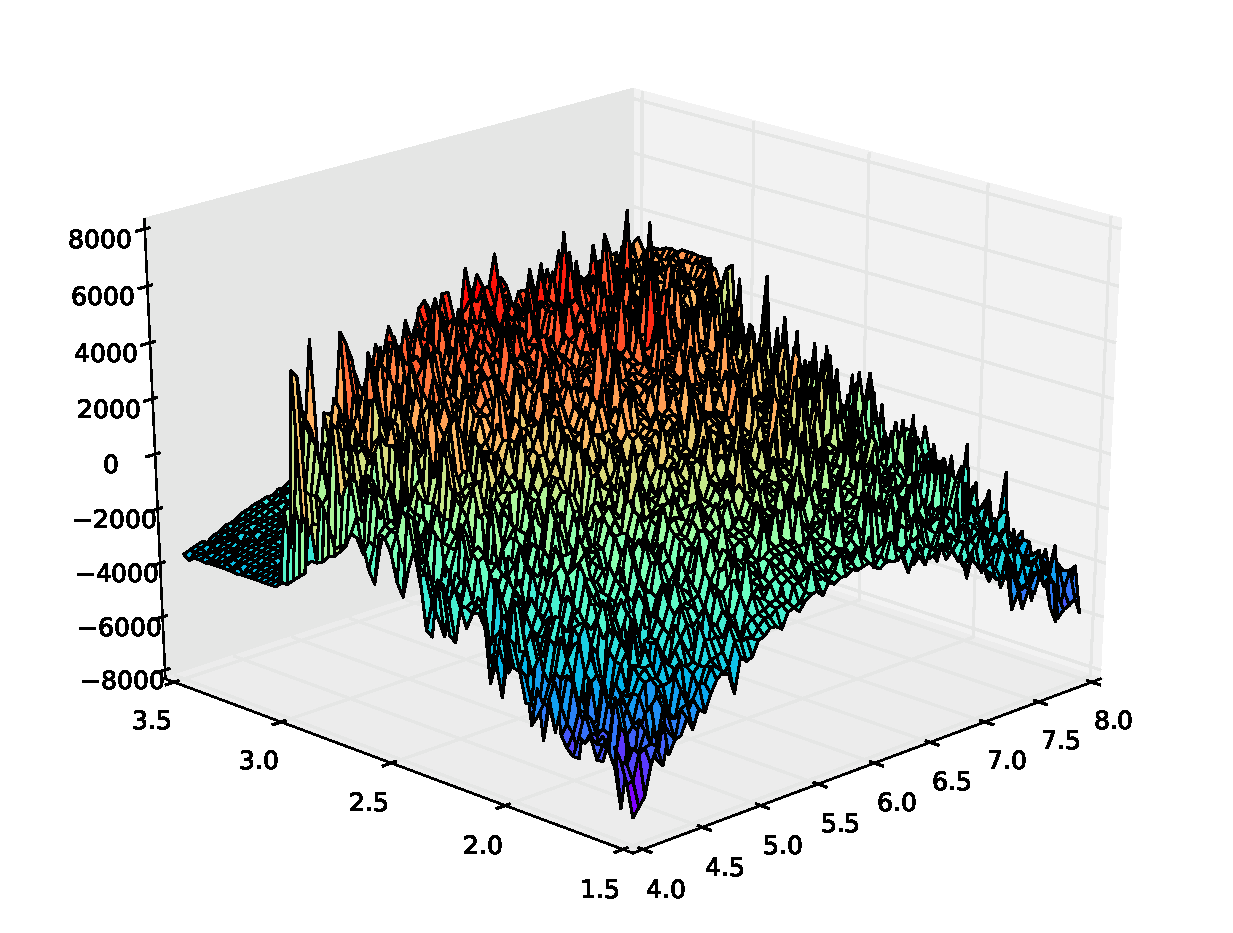
\includegraphics[width=0.75\textwidth]{figures/p1p2figure.eps}
\caption{最优$p_1, p_2$仿真结果}\label{fig:simuP1P2Result}
\vspace{-1em}
\end{figure}

\section{代码环境}

很多和计算机专业背景相关的同学都会使用到代码环境,使用~\verb|\verb|~指令或者是~\verb|verbatim|~环境固然是一种选择,但是比不上专门的~lstlisting~环境这么专业。

\begin{lstlisting}
int main(int argc, char ** argv) {
    printf("Hello world!\n");
    return 0;
}
\end{lstlisting}

\section{普通表格的绘制方法}

表格应具有三线表格式,其标准格式如表 \ref{tab:table1} 所示。
\begin{table}[htbp]
\caption{符合本科生毕业论文绘图规范的表格}\label{tab:table1}
\vspace{0.5em}\centering\wuhao
\begin{tabular}{ccccc}
\toprule[1.5pt]
$D$(in) & $P_u$(lbs) & $u_u$(in) & $\beta$ & $G_f$(psi.in)\\
\midrule[1pt]
 5 & 269.8 & 0.000674 & 1.79 & 0.04089\\
10 & 421.0 & 0.001035 & 3.59 & 0.04089\\
20 & 640.2 & 0.001565 & 7.18 & 0.04089\\
 5 & 269.8 & 0.000674 & 1.79 & 0.04089\\
10 & 421.0 & 0.001035 & 3.59 & 0.04089\\
20 & 640.2 & 0.001565 & 7.18 & 0.04089\\
 5 & 269.8 & 0.000674 & 1.79 & 0.04089\\
10 & 421.0 & 0.001035 & 3.59 & 0.04089\\
20 & 640.2 & 0.001565 & 7.18 & 0.04089\\
 5 & 269.8 & 0.000674 & 1.79 & 0.04089\\
10 & 421.0 & 0.001035 & 3.59 & 0.04089\\
20 & 640.2 & 0.001565 & 7.18 & 0.04089\\
\bottomrule[1.5pt]
\end{tabular}
\vspace{\baselineskip}
\end{table}

%%%%%%%%%%  参考文献  %%%%%%%%%%
\makereferences

%%%%%%%%%%    附录    %%%%%%%%%%
\titleformat{\chapter}{\centering\sihao\hei}{\chaptername}{2em}{}
\chapter*{\centering\xiaosan\hei 附\qquad 录}
\addcontentsline{toc}{chapter}{附\quad 录}       % 参考文献加入到中文目录
请插入各种附件。

2021年3月20日补充:请按照XeLaTex,BibTex,XeLaTex,XeLaTex的顺序编译(才能显示参考文献和各种引用)。

%%%%%%%%%%    致谢    %%%%%%%%%%
% !Mode:: "TeX:UTF-8"

%\titlecontents{chapter}[2em]{\vspace{.5\baselineskip}\xiaosan\song}
%             {\prechaptername\CJKnumber{\thecontentslabel}\postchaptername\qquad}{} 
%           %  {}                            % 设置该选项为空是为了不让目录中显示页码
%\chapter*{\centering\xiaosan\hei 致\qquad 谢}
\markboth{致\quad 谢}{致\quad 谢}
\addcontentsline{toc}{chapter}{致\quad 谢} % 添加到目录中
\chapter*{致\qquad 谢}

tjuthesis 的原作者们作出了前人栽树的不可磨灭的贡献:\\
* 张井 天津大学2010级管理与经济学部信息管理与信息系统专业硕士生\\
* 余蓝涛 天津大学2008级精密仪器与光电子工程学院测控技术与仪器专业本科生\\
以及北京大学孟祥溪院士。

~

~

2021年3月20日补充:本模板由2017级物理系本科生李佩璇在前人的基础上,参照天津大学最新论文模板修改。若有问题请联系邮箱lipeixuan@tju.edu.cn。            % 致谢
\clearpage
\end{document}                                 % 结束全文
